\documentclass[11pt,a4paper]{article}
\usepackage[utf8]{inputenc}
\usepackage[italian]{babel}
\usepackage{geometry}
\usepackage[font=small,labelfont=bf]{caption}
\geometry{left=3.5cm,right=3.5cm,top=3.0cm,bottom=2.5cm}
\usepackage[table,xcdraw]{xcolor}
\usepackage{longtable}
\usepackage{soulutf8}
\usepackage{fancyhdr}
\usepackage{tikz}
\usepackage{pgfkeys}
\usetikzlibrary{calc}
\usepackage{pgfplots}
\pgfplotsset{compat=newest}
\usepackage{pdfpages}
\usepackage{lastpage}
\usepackage{float}
\usepackage{listings}
\usepackage{eurosym}
\usepackage{enumitem}

%Pacchetto per permettere il riferimento a url e elementi interni ai documenti. Aggiunto da Davide in data 13-12-18
\usepackage{hyperref}

\hypersetup{
	colorlinks=true,
	linkcolor=black,
	urlcolor=blue
}
% ==================================================================================================
% COMANDI DA RIDEFINIRE
% ==================================================================================================

% Nome/Versione/Data del documento
\newcommand{\documentName}{ERRORE}
\newcommand{\documentVersion}{ERRORE}
\newcommand{\documentDate}{ERRORE}

% Editori del documento
\newcommand{\documentEditors}{ERRORE}

% Verificatore del documento
\newcommand{\documentVerifiers}{ERRORE}

% Approvatore del documento
\newcommand{\documentApprovers}{ERRORE}

% Uso del documento
\newcommand{\documentUsage}{ERRORE}

% Destinatari del documento
\newcommand{\documentAddressee}{ERRORE}

% Sommario del documento
\newcommand{\documentSummary}{ERRORE}

% Vesione dei documenti
\newcommand{\docVersionGlo}{\textit{v1.0.0}} % Glossario
\newcommand{\docVersionNdP}{\textit{v1.0.0}} % Norme di Progetto
\newcommand{\docVersionSdF}{\textit{v1.0.0}} % Studio di Fattibilità
\newcommand{\docVersionPdP}{\textit{v1.0.0}} % Piano di Progetto
\newcommand{\docVersionPdQ}{\textit{v1.0.0}} % Piano di Qualifica
\newcommand{\docVersionST}{\textit{v1.0.0}} % Specifica Tecnica
\newcommand{\docVersionDdP}{\textit{v1.0.0}} % Definizione di Prodotto
\newcommand{\docVersionAdR}{\textit{v1.0.0}} % Analisi dei Requisiti
\newcommand{\docVersionMU}{\textit{v1.0.0}} % Manuale Utente
\newcommand{\docVersionMS}{\textit{v1.0.0}} % Manuale Sviluppatore

% ==================================================================================================
% COMANDI DA NON RIDEFINIRE
% ==================================================================================================

% Stile font
\newcommand{\code}[1]{\texttt{\textbackslash{}#1}} % Testo stile codice
\newcommand{\glo}{\ped{\textbf{\tiny G}}} % Testo glossario
\newcommand{\es}[1]{(e.g. #1)} % Esempio e.g.

% Nome del progetto
\newcommand{\projectName}{ShopChain}
\newcommand{\groupEmail}{\textit{\href{mailto:yakuzaishi.swe@gmail.com}{yakuzaishi.swe@gmail.com}}}
\newcommand{\groupName}{Yakuzaishi}

% Componenti del gruppo
\newcommand{\team}{Francesco Bugno, Luca Busacca, Luca Carturan, Michele Filosofo, Dario Furlan, Francesco Mattarello, Matteo Midena}

% Ruoli del progetto
\newcommand{\roleProjectManager}{\textit{Responsabile}}
\newcommand{\roleAdministrator}{\textit{Amministratore}}
\newcommand{\roleAnalyst}{\textit{Analista}}
\newcommand{\roleProgrammer}{\textit{Programmatore}}
\newcommand{\roleDesigner}{\textit{Progettista}}
\newcommand{\roleVerifier}{\textit{Verificatore}}

% Referenti e commitenti
\newcommand{\proposerName}{Fabio Pallaro - Sync Lab S.r.l.}
\newcommand{\commitNameM}{Prof. Tullio Vardanega}
\newcommand{\commitNameS}{Prof. Riccardo Cardin}

% Nome dei documenti
\newcommand{\docNameGlo}{\textit{Glossario}} % Glossario
\newcommand{\docNameNdP}{\textit{Norme di Progetto}} % Norme di Progetto
\newcommand{\docNameSdC}{\textit{Studio dei Capitolati}} % Studio dei Capitolati
\newcommand{\docNameST}{\textit{Specifica Tecnica}} % Specifica Tecnica
\newcommand{\docNameDdP}{\textit{Definizione di Prodotto}} % Definizione di Prodotto
\newcommand{\docNamePdP}{\textit{Piano di Progetto}} % Piano di Progetto
\newcommand{\docNamePdQ}{\textit{Piano di Qualifica}} % Piano di Qualifica
\newcommand{\docNameAdR}{\textit{Analisi dei Requisiti}} % Analisi dei Requisiti
\newcommand{\docNameMU}{\textit{Manuale Utente}} % Manuale Utente
\newcommand{\docNameMS}{\textit{Manuale Sviluppatore}} % Manuale Sviluppatore
\newcommand{\docNameI}{\textit{Impegni}} % Impegni

% Nome e versione dei documenti
\newcommand{\docNameVersionGlo}{\docNameGlo{} \docVersionGlo} % Glossario
\newcommand{\docNameVersionNdP}{\docNameNdP{} \docVersionNdP} % Norme di Progetto
\newcommand{\docNameVersionSdF}{\docNameSdF{} \docVersionSdF} % Studio dei Capitolati
\newcommand{\docNameVersionPdP}{\docNamePdP{} \docVersionPdP} % Piano di Progetto
\newcommand{\docNameVersionPdQ}{\docNamePdQ{} \docVersionPdQ} % Piano di Qualifica
\newcommand{\docNameVersionAdR}{\docNameAdR{} \docVersionAdR} % Analisi dei Requisiti
\newcommand{\docNameVersionMU}{\docNameMU{} \docVersionMU} % Manuale Utente
\newcommand{\docNameVersionMS}{\docNameMS{} \docVersionMS} % Manuale Sviluppatore

% Nome delle revisioni
\newcommand{\RTB}{\textit{Requirements and Technology Baseline}}
\newcommand{\PB}{\textit{Product Baseline}}
\newcommand{\CA}{\textit{Customer Acceptance}}

% Descrizione del glossario
\newcommand{\gloDesc}{I termini utilizzati in questo documento potrebbero generare dubbi riguardo al loro significato, richiedendo pertanto una definizione al fine di evitare ambiguità.\\Tali termini vengono contrassegnati da una G maiuscola finale a pedice della parola.\\La loro spiegazione è riportata nel \docNameVersionGlo{}.}
\fancypagestyle{styleDocPages}{
	\thispagestyle{empty}
	\thispagestyle{fancy}
	\pagestyle{fancy}
	% HEADER
	\setlength{\topmargin}{-40pt}
	\setlength{\headsep}{60pt}
	\fancyhf{}
	\lhead{Yakuzaishi}
	\setlength{\headheight}{15pt}
	\rhead{
\includegraphics[width=1cm]{../template/images/logo_header}}
	
	% FOOTER
	\fancyfoot{}
	\fancyfoot[L]{\documentName}
	\fancyfoot[R]{Pagina \thepage~di~\pageref{LastPage}}
	\futurelet\TMPfootrule\def\footrule{\TMPfootrule}
	\setcounter{page}{0}
	\pagenumbering{arabic}
	\renewcommand{\footrulewidth}{0.3pt}
}

\setcounter{secnumdepth}{5}
\setcounter{tocdepth}{5}

\setcounter{tocdepth}{5}	%aggiunge paragrafi e sottoparagrafi all'indice
\setcounter{secnumdepth}{5}	%aggiunge numero indicizazzione a paragrafi e sottoparagrafi

%indentazione sottoparagrafi
\makeatletter
\renewcommand\subparagraph{
\@startsection {subparagraph}{5}{0mm}{-\baselineskip}{.5\baselineskip}{\normalfont \normalsize \bfseries }}
\makeatother

\begin{document}
	%RIDEFINIZIONE COMANDI
	%%%%%%%%%%%%%%%%%%%%%%%%%%%%%%%%%%%%%%%%%%%%%%%%%%%%%%%%%%%%%%%
	\renewcommand{\documentName}{Norme di Progetto}
	\renewcommand{\documentVersion}{2.0.0}
	
	\renewcommand{\documentApprovers}{Francesco Mattarello}
	\renewcommand{\documentEditors}{Luca Carturan\\&Michele Filosofo}
	\renewcommand{\documentVerifiers}{Matteo Midena}
	
	\renewcommand{\documentUsage}{Interno}
	\renewcommand{\documentAddressee}{\commitNameM\\&\commitNameS\\&\proposerName}
	\renewcommand{\documentSummary}{Questo documento raccoglie le regole, gli strumenti e le convenzioni adottate dal gruppo Yakuzaishi definendone il \textit{way of working}.}
	%%%%%%%%%%%%%%%%%%%%%%%%%%%%%%%%%%%%%%%%%%%%%%%%%%%%%%%%%%%%%%%
	
	%PRIMA PAGINA
	%%%%%%%%%%%%%%%%%%%%%%%%%%%%%%%%%%%%%%%%%%%%%%%%%%%%%%%%%%%%%%%
	\pagenumbering{gobble}
	\pagestyle{empty}
	\thispagestyle{empty}

%Logo gruppo
\begin{figure}
	\centering
	
\includegraphics[width=150px]{../template/images/logo}
\end{figure}

\hspace{5pt}

%Nome documento
\begin{center}
	\textbf{\Large \documentName}\\[0.2cm]
%	\textbf{\Large Progetto \projectName}
\end{center}

\vspace{5pt}

%Email
\begin{center}
	\groupEmail
\end{center}

\vspace{5pt}

%Informazioni documento
\begin{center}
	\textbf{Informazioni sul documento}
\end{center}

\begin{table}[H]
	\centering
	\renewcommand{\arraystretch}{1.4}
	\begin{tabular}{r|l}
		Responsabile & \documentApprovers\vspace{2.5pt}\\
		Redattori & \documentEditors\vspace{2.5pt}\\
		Verificatori & \documentVerifiers\vspace{2.5pt}\\
		Uso & \documentUsage\vspace{2.5pt}\\
		Destinatari & \documentAddressee\\
	\end{tabular}
\end{table}

\vspace{40pt}

%Sommario
\begin{center}
	\textbf{Sommario}\\
	\documentSummary
\end{center}

\tikz[remember picture,overlay] \node[opacity=0.2,inner sep=0pt] at (current page.center){
\includegraphics[width=\paperwidth,height=\paperheight]{../template/images/sfondo}};
	\pagebreak
	%%%%%%%%%%%%%%%%%%%%%%%%%%%%%%%%%%%%%%%%%%%%%%%%%%%%%%%%%%%%%%%
	
	%CHANGELOG E INDICI
	%%%%%%%%%%%%%%%%%%%%%%%%%%%%%%%%%%%%%%%%%%%%%%%%%%%%%%%%%%%%%%%
	\thispagestyle{empty}
\section*{Registro delle Modifiche}

\begin{center}
	\renewcommand{\arraystretch}{1.8}
	\rowcolors{2}{green!100!black!40}{green!100!black!30}
	\begin{longtable}[c]{c | c | c | c | p{5cm}}
		\rowcolor[HTML]{125E28}
		\multicolumn{1}{c}{\color[HTML]{FFFFFF} \textbf{Versione}} & 
		\multicolumn{1}{c}{\color[HTML]{FFFFFF} \textbf{Data}} & 
		\multicolumn{1}{c}{\color[HTML]{FFFFFF} \textbf{Autore}} & 
		\multicolumn{1}{c}{\color[HTML]{FFFFFF} \textbf{Ruolo}} & 
		\multicolumn{1}{c}{\color[HTML]{FFFFFF} \textbf{Descrizione}} \\
		\endhead
		1.0.0 & 2021/11/11 & Francesco Mattarello & Responsabile & Approvato per il rilascio\\
		0.2.0 & 2021/11/07 & Matteo Midena & Verificatore & Verifica modifiche §\ref{subsection:gestione}\\
		0.1.1 & 2021/11/07 & Luca Carturan & Analista & Modifiche §\ref{subsection:gestione}\\
		0.1.0 & 2021/11/06 & Matteo Midena & Verificatore & Verifica  §\ref{subsection:gestione} e  §\ref{subsection:infrastrutture_interne}\\
		0.0.2 & 2021/11/05 & Michele Filosofo & Analista & Stesura §\ref{subsection:infrastrutture_interne}\\
		0.0.1 & 2021/11/04 & Luca Carturan & Analista &Stesura §\ref{subsection:gestione}  \\

	\end{longtable}
\end{center} \pagebreak
	\renewcommand{\contentsname}{Contenuti}
	\tableofcontents \pagebreak
	%\listoftables \pagebreak
	%\listoffigures \pagebreak
	%%%%%%%%%%%%%%%%%%%%%%%%%%%%%%%%%%%%%%%%%%%%%%%%%%%%%%%%%%%%%%%
	
	%CONTENUTO
	%%%%%%%%%%%%%%%%%%%%%%%%%%%%%%%%%%%%%%%%%%%%%%%%%%%%%%%%%%%%%%%
	\pagestyle{styleDocPages}
	%Contenuto del documento
\section{Introduzione}\label{section:introduzione}

\subsection{Scopo del documento}
In questa sezione viene riportato il preventivo per il progetto, suddividendo le ore di lavoro e i costi.
La suddivisione oraria dei ruoli per ogni membro del gruppo dovrà rispettare le seguenti regole:
\begin{itemize}
	\item ogni componente dovrà ricoprire almeno una volta ogni ruolo per almeno otto ore, in modo che tutti i componenti apprendano le attività e le responsabilità legate ai diversi ruoli;
	\item le ore lavorative per ogni fase dovranno essere le stesse per ogni componente, per far si che tutti apportino lo stesso contributo al progetto, senza alcuna differenza.
\end{itemize}
Per riportare i ruoli nelle tabelle, essi sono abbreviati con le seguenti sigle:
\begin{itemize}
	\item\textbf{Re:} Responsabile;
	\item\textbf{Am:} Amministratore;
	\item\textbf{An:} Analista;
	\item\textbf{Pg:} Progettista;
	\item\textbf{Pr:} Programmatore;
	\item\textbf{Ve:} Verificatore.
\end{itemize}




\section{Tecnologie coinvolte}


\begin{table}[H]
	\centering
	\renewcommand{\arraystretch}{1.8}
	\rowcolors{2}{green!100!black!40}{green!100!black!30}
	\begin{tabular}{c | c | c}
		\rowcolor[HTML]{125E28}
		\multicolumn{1}{c}{\color[HTML]{FFFFFF} \textbf{Tecnologia}} &
        \multicolumn{1}{c}{\color[HTML]{FFFFFF} \textbf{Versione}} & 
		\multicolumn{1}{c}{\color[HTML]{FFFFFF} \textbf{Descrizione}}   \\ \hline
        \rowcolor[HTML]{1c9c3e}
        \multicolumn{3}{c}{\color[HTML]{FFFFFF} \textbf{Linguaggi}} \\ \hline
        Typescript & 4.6.3 & Linguaggio fortemente tipato, basato su Javascript, più scalabile \\ \hline
        Solidity & 1.0 & \shortstack{Linguaggio usato per la creazione di Smartcontracts su varie blockchain,\\ in particolare tutte quelle basate su Ethereum} \\ \hline
        HTML & 5 & \shortstack{Utilizzato nel progetto assieme a React\\ per definire l’interfaccia grafica} \\ \hline
        Sass & 1.47.0 & \shortstack{Estensione di CSS, utilizzato per definire\\ la formattazione dei documenti HTML5 e lo stile} \\ \hline
        \rowcolor[HTML]{1c9c3e}
        \multicolumn{3}{c}{\color[HTML]{FFFFFF} \textbf{Strumenti}} \\ \hline
        Npm & 7.x & \shortstack{Gestore di pacchetti utilizzato per effettuare\\ le operazioni di build del codice} \\ \hline
        Babel & 7.9.6 & \shortstack{Transcompiler JavaScript utilizzato per convertire il codice \\ECMAScript 2015+ in una versione retro compatibile per \\browser non aggiornati} \\ \hline
        Truffle & 5.4.33 & \shortstack{Ambiente di test locale per Smartcontract} \\ \hline
        Docker & 4.9.0 & \shortstack{Strumento open-source che automatizza\\ il processo di deployment di applicazioni\\ all'interno di contenitori software} \\ \hline
        \rowcolor[HTML]{1c9c3e}
        \multicolumn{3}{c}{\color[HTML]{FFFFFF} \textbf{Librerie}} \\ \hline
        React & 16.3.1 & \shortstack{Libreria per la creazione di UI scelta per facilitare lo\\ sviluppo del front-end e avere performance migliori grazie \\al suo metodo di renderizzazione dei componenti grafici} \\ \hline
        MobX & 6.5 & \shortstack{Libreria per React che permette la gestione dello stateG dei \\componenti e l’implementazione del design pattern \\Observer} \\ \hline
        Web3.js & 1.7.0 & \shortstack{Collezione di librerie per interagire con nodi ethereum locali o remoti} \\ \hline
        %%%%%%%%%%%%%%%%%%%%%%%%%%%%%% TO BE COMPLETED %%%%%%%%%%%%%%%%%%%%%%%%%%%%%%%%%%%%%%%%%%%%%%%%%%%
    \end{tabular}
    \caption{Tabella delle tecnologie}
\end{table}

%% react 16.3.1 web3 1.7.0 mobX 6.5 babel 7.9.6 sass 1.47.0 html 5 jest 27.5.1 solidity 0.8.11 chai 4.3.6 mocha 9.2.0 truffle 5.4.33
\section{Setup}\label{section:setup}

In questa sezione vengono trattati i requisiti minimi necessari per l’utilizzo dell’applicazione ShopChain e successivamente come poter installare il prodotto in locale direttamente dal repository\glo
pubblico GitHub\glo del gruppo Yakuzaishi, accessibile al seguente link: \href{https://yakuzaishi-swe.github.io}{link al repository}.

\subsection{Requisiti di sistema}

Per far si che le operazioni di installazione e avvio del prodotto avvengano correttamente e che si possa
aver accesso a tutte le funzionalità, è necessario avere installati nella propria macchina i seguenti software.

\begin{table}[H]
	\centering
	\renewcommand{\arraystretch}{1.8}
	\rowcolors{2}{green!100!black!40}{green!100!black!30}
    \begin{tabular}{c | c | c}
		\rowcolor[HTML]{125E28}
		\multicolumn{1}{c}{\color[HTML]{FFFFFF} \textbf{Software}} &
        \multicolumn{1}{c}{\color[HTML]{FFFFFF} \textbf{Versione}} & 
		\multicolumn{1}{c}{\color[HTML]{FFFFFF} \textbf{Link al download}}   \\ \hline
        Docker & 4.9.0 & \href{https://www.docker.com/products/docker-desktop/}{https://www.docker.com/products/docker-desktop/} \\ \hline
    \end{tabular}
    \caption{Requisiti di sistema}
\end{table}

Grazie all'utilizzo di Docker\glo, abbiamo facilitato la procedura di setup dell'applicazione, in quanto Docker stesso si occupa di inizializzare tutte le tecnologie necessarie alla compilazione.

\subsection{Requisiti hardware}

Per avere delle prestazioni accettabili dell’applicazione è preferibile possedere almeno i seguenti componenti hardware.

\begin{table}[H]
	\centering
	\renewcommand{\arraystretch}{1.8}
	\rowcolors{2}{green!100!black!40}{green!100!black!30}
    \begin{tabular}{c | c}
		\rowcolor[HTML]{125E28}
		\multicolumn{1}{c}{\color[HTML]{FFFFFF} \textbf{Componente}} &
		\multicolumn{1}{c}{\color[HTML]{FFFFFF} \textbf{Requisito}}   \\ \hline
        RAM & 4GB DDR4 \\ \hline
        CPU & Processore 64-bit con Second Level Address Translation \href{https://en.wikipedia.org/wiki/Second_Level_Address_Translation}{(SLAT)} \\ \hline
        SSD (o HDD) & 3GB \\ \hline
    \end{tabular}
    \caption{Requisiti hardware}
\end{table}

\underline{\textbf{Attenzione!}} In alcune CPU la virtualizzazione utilizzata da Docker per avviarsi non è abilitata di default, per abilitarla si deve accedere al BIOS\glo di sistema, e attivare l'impostazione correlata.
Essend i BIOS molto variabili da macchina a macchina, non ci è possibile dare una indicazione precisa su dove trovare l'impostazione da cambiare, al seguente link troverete una guida generale di esempio: \href{https://www.bleepingcomputer.com/tutorials/how-to-enable-cpu-virtualization-in-your-computer-bios/}{CPU virtualization}.

È necessaria inoltre una connessione internet stabile per garantire un servizio ottimale, senza vincoli di banda.

\subsection{Browser}

L’applicazione è stata testata e quindi resa compatibile con le ultime versioni dei browser che supportano l'estensione Metamask\glo, il cui setup verrà discusso nella sezione §\ref{subsection:Metamask}.

\begin{table}[H]
	\centering
	\renewcommand{\arraystretch}{1.8}
	\rowcolors{2}{green!100!black!40}{green!100!black!30}
    \begin{tabular}{c | c}
    \rowcolor[HTML]{125E28}
	\multicolumn{1}{c}{\color[HTML]{FFFFFF} \textbf{Componente}} &
	\multicolumn{1}{c}{\color[HTML]{FFFFFF} \textbf{Requisito}}   \\ \hline
    Google Chrome & 98 \\ \hline
    Microsoft Edge & 98 \\ \hline
    Mozilla Firefox & 97 \\ \hline
    Brave Browser & 1.36 \\ \hline
    \end{tabular}
    \caption{Requisiti browser}
\end{table}

\subsection{Metamask} \label{subsection:Metamask}

L'applicazione fa uso del plugin Metamask\glo per la gestione dei wallet e dei pagamenti, 
al seguente link è possibile trovare la pagina ufficiale di download:
 \begin{center}
     \url{https://MetaMask.io/download/}
 \end{center}
 Alla pagina sarà presente un bottone con scritto \texttt{"Install MetaMask"}
 \begin{figure}[H]
    \centering
    \includegraphics[scale=0.3]{immagini/install-MetaMask.png}
    \caption{Pagina download MetaMask}
\end{figure}
\textbf{}\\
Cliccando il bottone si verrà reindirizzati alla seguente pagina web nella quale basterà cliccare il bottone \textit{"Aggiungi"}:
\begin{figure}[H]
    \centering
    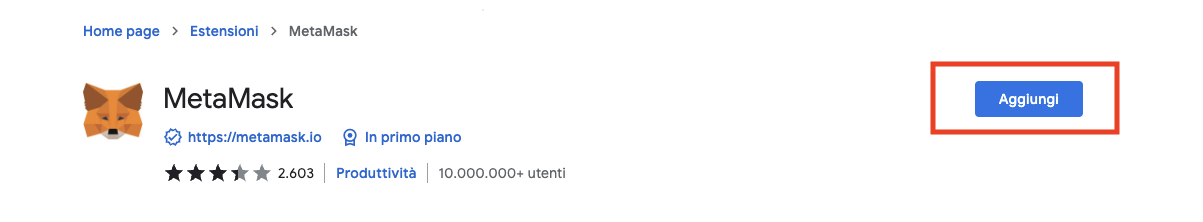
\includegraphics[scale=0.3]{immagini/MetaMaskExtensionPage.png}
    \caption{Aggiungere l'estensione MetaMask al browser (1)}
\end{figure}
\textbf{}\\
Si aprirà dunque il popup mostrato in seguito nel quale sarà sufficiente cliccare \texttt{"Aggiungi estensione"}
\begin{figure}[H]
    \centering
    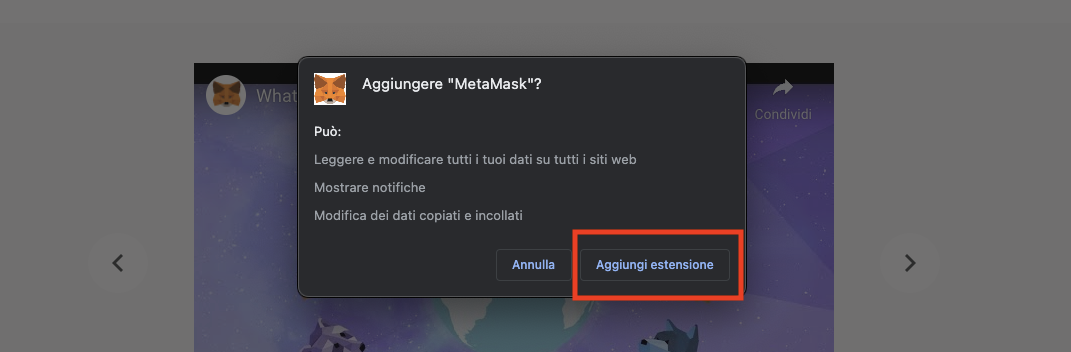
\includegraphics[scale=0.3]{immagini/AddExtenction.png}
    \caption{Aggiungere l'estensione MetaMask al browser (2)}
\end{figure}
\textbf{}\\
Una volta che l'estensione sarà stata aggiunta si verrà automaticamente reindirizzati alla pagina mostrata nella figura seguente nella quale sarà sufficiente cliccare \textit{Inizia}
\begin{figure}[H]
    \centering
    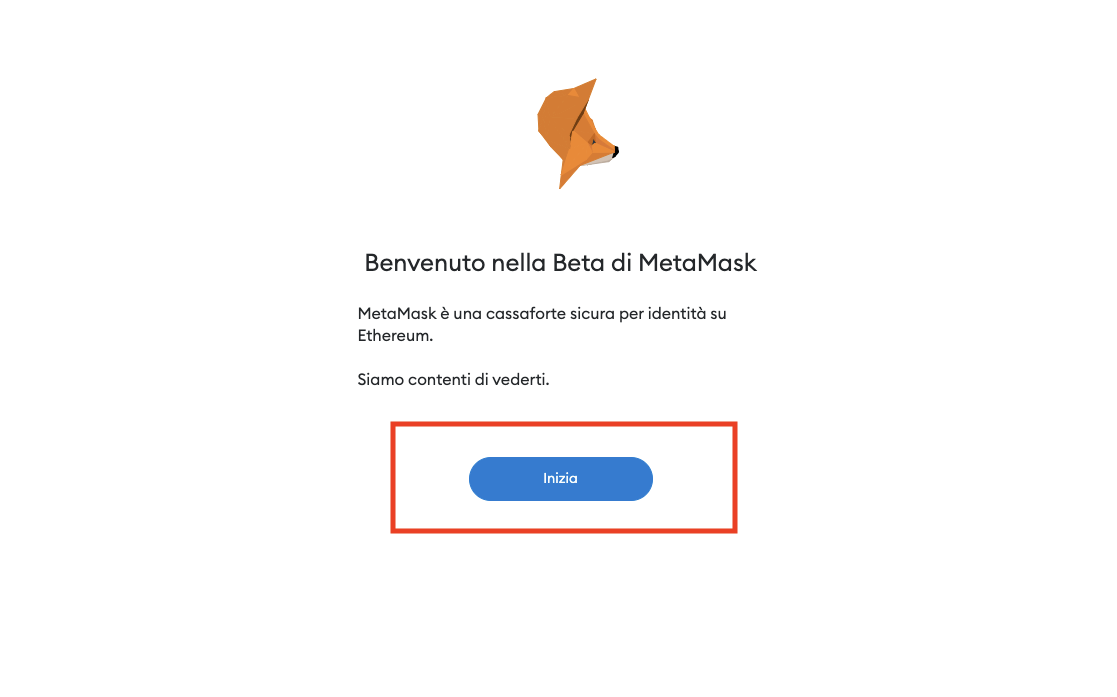
\includegraphics[scale=0.3]{immagini/startMetamask.png}
    \caption{Pagina iniziale MetaMask}
\end{figure}

\textbf{}\\
A questo punto non resta che scegliere se iniziare creando un nuovo portafoglio o se caricarne uno già esistente.

\begin{figure}[H]
    \centering
    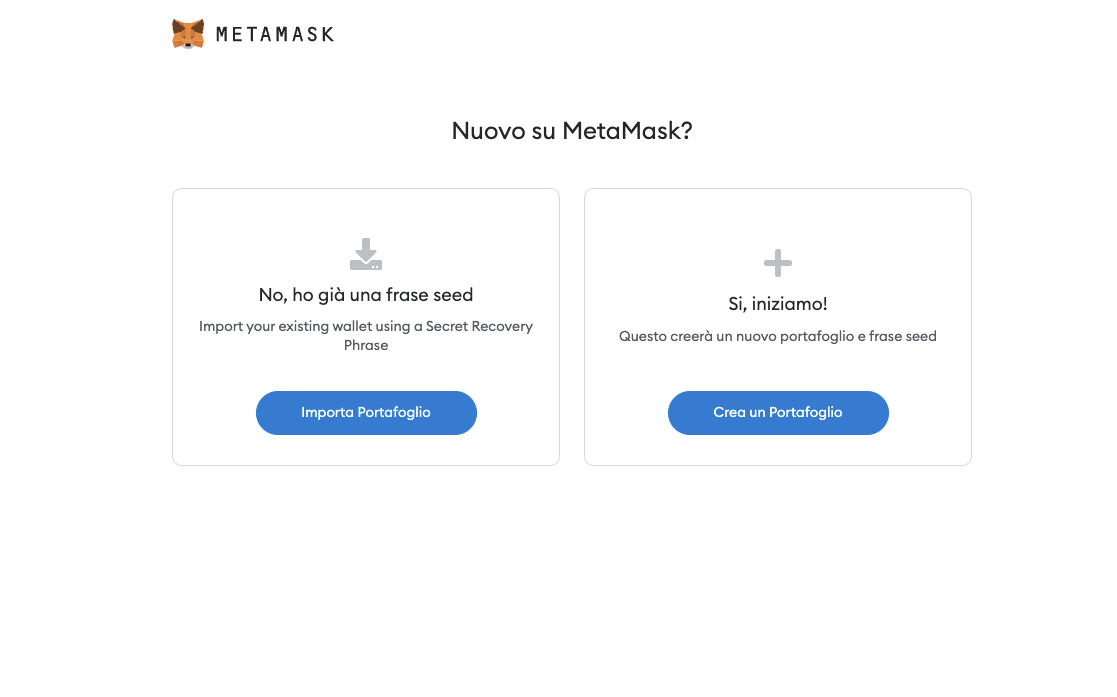
\includegraphics[scale=0.3]{immagini/chooseMetamask.png}
    \caption{Scelta iniziale MetaMask: crea/importa portafogli}
\end{figure}

\textbf{}\\
dopo aver scelto basterà seguire le semplici istruzioni riportate da MetaMask per completare il collegamento.

\subsubsection{Configurazione}
Per utilizzare l'applicazione \projectName{} è necessario disporre di un account MetaMask impostato sulla testnet Fantom.
Per aggiungere una nuova rete al proprio account MetaMask, cliccare sull'estensione MetaMask, quindi su \texttt{"Rete Ethereum Principale"}  e infine \texttt{"Aggiungi Rete"} come mostrato di seguito:
\begin{figure}[H]
    \centering
    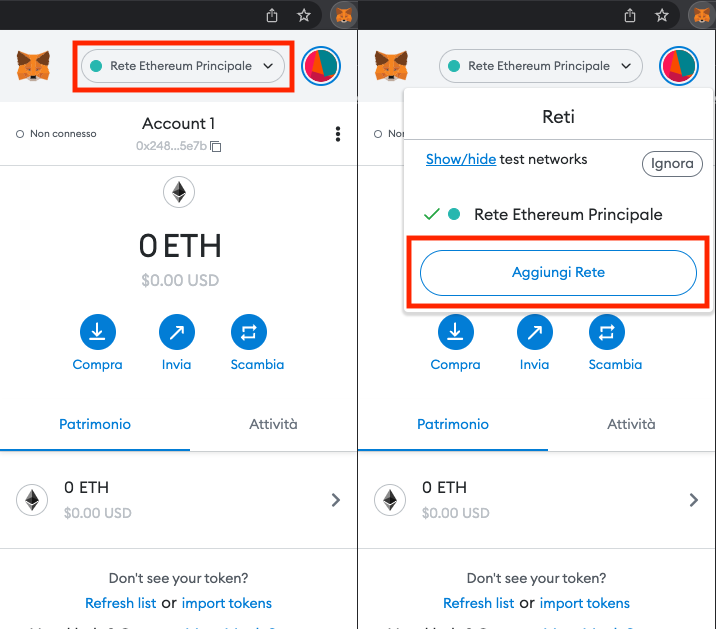
\includegraphics[scale=0.4]{immagini/Configuration.png}
    \caption{Inizio configurazione Fantom Testnet}
\end{figure}
\textbf{}\\
Si verrà reindirizzati a una pagina contenente un form da riempire come mostrato di seguito:
\begin{figure}[H]
    \centering
    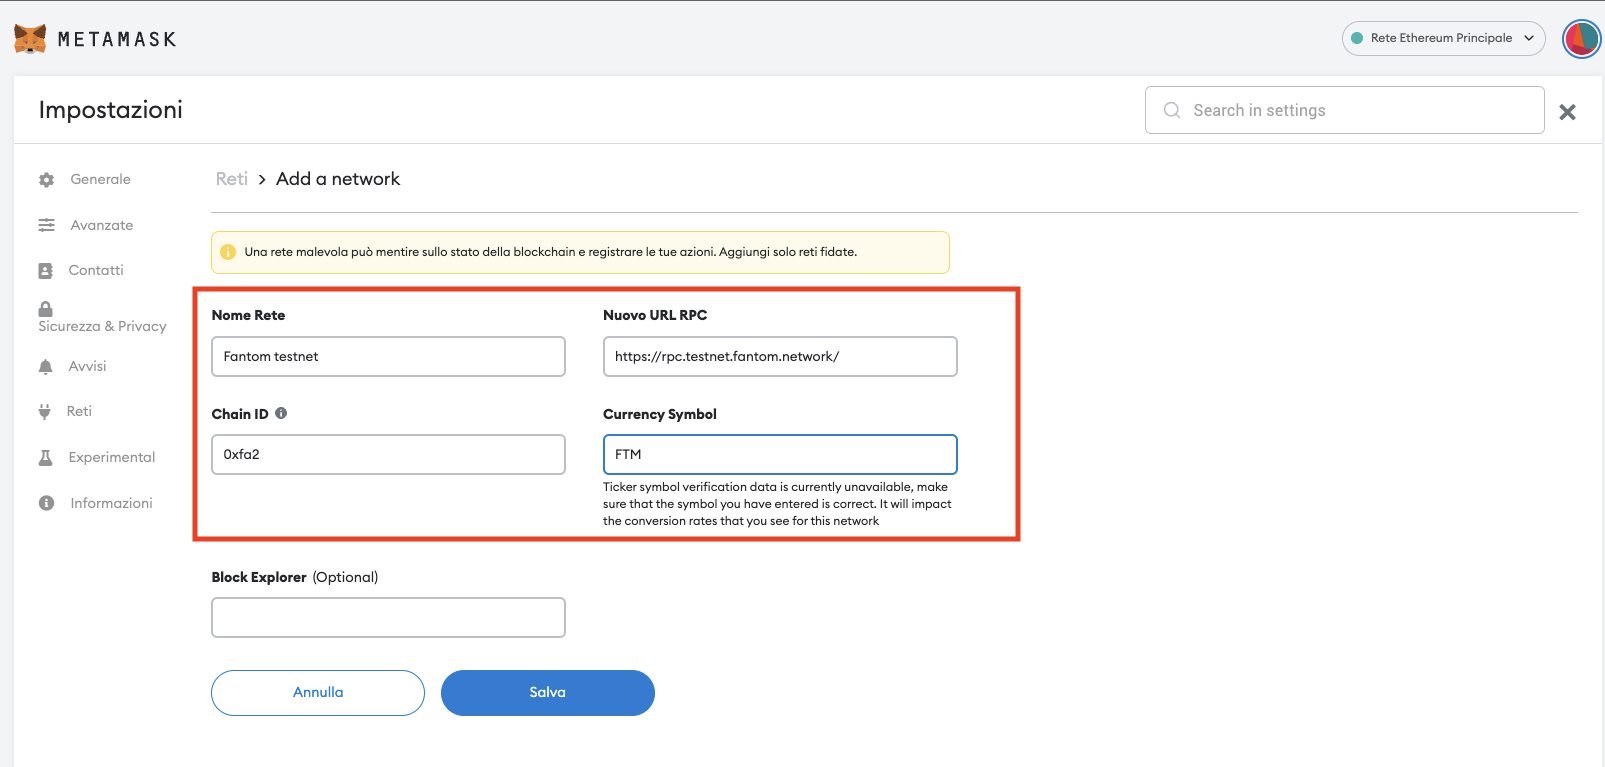
\includegraphics[scale=0.3]{immagini/ConfData.png}
    \caption{Form per l'aggiunta della rete Fantom Testnet}
\end{figure} 
\textbf{}\\
Per comodità vengono riportati i dati:
\begin{itemize}
    \item Network Name: Fantom testnet;
    \item New RPC Url: https://rpc.testnet.fantom.network/;
    \item ChainID: 0xfa2
    \item Symbol: FTM
\end{itemize}
Una volta riempito il form cliccare il tasto \texttt{Salva}.\\
A questo punto, una volta caricato denaro nel portafogli tramite la \href{https://faucet.fantom.network/}{Fantom faucet}, il setup sarà completo.\\\\
\underline{\textbf{Attenzione!}} Si raccomanda inoltre di notare che ciascuna operazione che prevede l'interazione con MetaMask (quali il pagamento, lo sblocco, il rimborso, la creazione della moneybox e il versamento di un contributo) prevedono il pagamento di gasfee, ovvero un ammontare variabile, generalmente piccolo, come commissione per il pagamento.\\
Tale ammontare è indipendente da \projectName{} o MetaMask, risulta invece essere indispensabile per permettere alla blockchain\glo{} di registrare i blocchi all'interno dei quali è possibile reperire le transazioni.
\section{Inizializzazione}\label{section:inizializzazione}

Per utilizzare l'applicazione web è necessario:
\begin{itemize}
    \item Clonare il repository;
    \item Installare le dipendenze;
    \item Avviare la web app.
\end{itemize}


\subsection{Clonare il repository}

\begin{enumerate}
    \item Scaricare il codice come file .zip direttamente dal repository shopchain-frontend:
            \begin{center}
                \href{https://github.com/Yakuzaishi-SWE/shopchain-frontend}{https://github.com/Yakuzaishi-SWE/shopchain-frontend}
            \end{center}
            Oppure, con Git\glo{} installato in locale, è possibile clonare il repository con il comando:
            \begin{center}
                \textcolor{red}{git clone https://github.com/Yakuzaishi-SWE/shopchain-frontend}
            \end{center}
    \item Se non clonato tramite Git, estrarre il file .zip.
\end{enumerate}

\subsection{Installare le dipendenze}

\begin{enumerate}
    \item Spostarsi all'interno del repository clonato tramite terminale con il comando:
    \begin{center}
        \textcolor{red}{cd percorso/shopchain-frontend}
    \end{center}
    \item Eseguire il comando:
    \begin{center}
        \textcolor{red}{npm i}
    \end{center}
    \item Attendere il termine della procedura di installazione delle dipendenze.
\end{enumerate}

\subsection{Avviare la web app}

\begin{enumerate}
    \item Dalla cartella, eseguire il comando:
    \begin{center}
        \textcolor{red}{npm start}
    \end{center}
    \item il browser di default si aprirà in automatico con l'applicativo eseguito.
\end{enumerate}
\section{Strumenti di analisi e integrazione del codice}\label{section:strumenti}

\begin{table}[H]
	\centering
	\renewcommand{\arraystretch}{1.8}
	\rowcolors{2}{green!100!black!40}{green!100!black!30}
	\begin{tabular}{c | c | c}
		\rowcolor[HTML]{125E28}
		\multicolumn{1}{c}{\color[HTML]{FFFFFF} \textbf{Strumento}} &
        \multicolumn{1}{c}{\color[HTML]{FFFFFF} \textbf{Versione}} & 
		\multicolumn{1}{c}{\color[HTML]{FFFFFF} \textbf{Descrizione}}   \\ \hline
        \rowcolor[HTML]{1c9c3e}
        \multicolumn{3}{c}{\color[HTML]{FFFFFF} \textbf{Analisi Statica}} \\ \hline
        ESLint & 8.9.0 & \shortstack{Strumento di analisi statica utilizzato per la segnalazione\\ degli errori di sintassi, per avere regole d'indentazione\\ uguali in tutti i file e per notifiche altri problemi comuni} \\ \hline
        \rowcolor[HTML]{1c9c3e}
        \multicolumn{3}{c}{\color[HTML]{FFFFFF} \textbf{Analisi Dinamica}} \\ \hline
        Jest & 27.5.1 & \shortstack{Framework javascript per il testing, creato appositamente per React} \\ \hline
        Chai & 4.3.6 & \shortstack{Libreria javascript per il testing} \\ \hline
        Mocha & 9.2.2 & \shortstack{Libreria javascript per il testing} \\ \hline
    \end{tabular}
    \caption{Strumenti per l'analisi e l'integrazione del codice}
\end{table}




\section{Architettura} \label{section:architettura}

Per lo sviluppo generale dell'applicazione, è stata seguita una architettura DApp\glo, (Fully) Decentralised Application.
Essa consiste in un frontend Web che effettua chiamate dirette ad una infrastruttura decentralizzata backend, nel 
nostro caso una gerarchia di smartcontracts eseguiti su blockchain Fantom; 
questa struttura ricorda quindi una architettura client-server, senza un supporto intermedio per le operazioni.
\\
\\
Il pattern architetturale\glo scelto dal gruppo per lo sviluppo del frontend è il Model-View-ViewModel\glo. Il
seguente pattern è tra i più diffusi nello sviluppo delle web application e permette di scrivere codice
facilmente mantenibile e riusabile; questo è possibile grazie al forte disaccoppiamento che sussiste tra
logica di presentazione e di business. Inoltre l'MVVM è risultato il più adatto per essere utilizzato con
React, libreria impiegata per lo sviluppo dell'UI e che renderizza le componenti in base al loro stato\glo\ interno.

\begin{figure}[H]
    \centering
    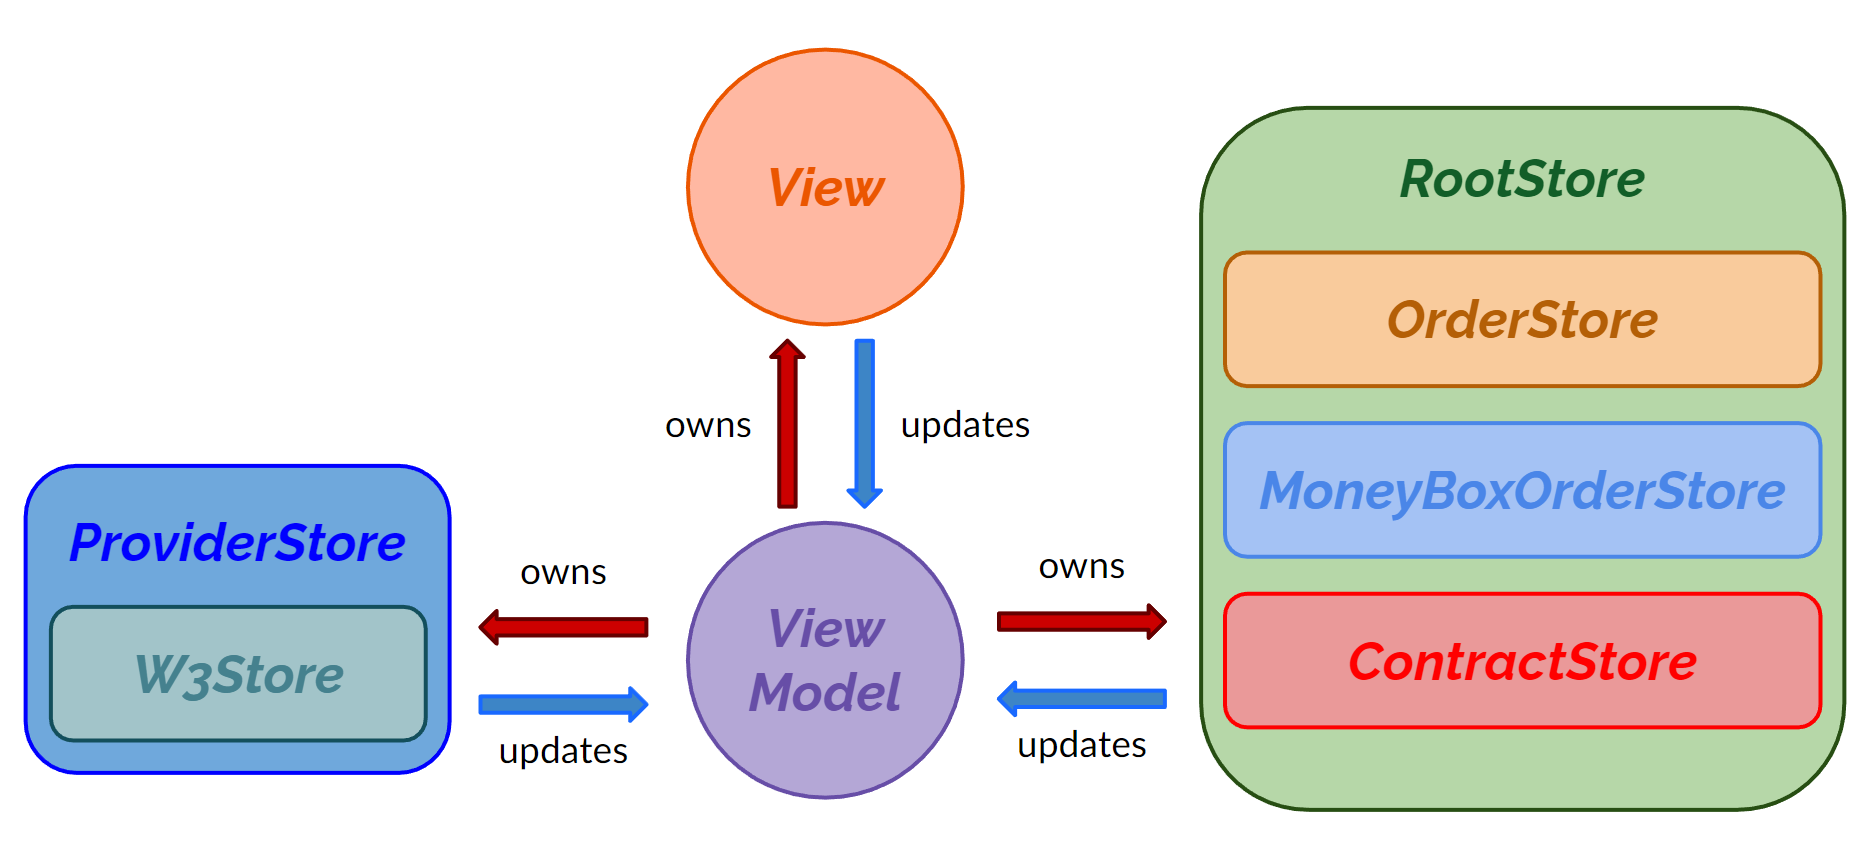
\includegraphics[scale=0.3]{immagini/mvvm.png}
    \caption{Model-View-ViewModel di ShopChain}
\end{figure}

Il passaggio dei dati dal Model alle varie componenti grafiche avviene attraverso l'utilizzo di un Context
React, al quale viene passato un'istanza del ViewModel. L'utilizzo di un Context React ci permette di
accedere al valore corrente del ViewModel in qualsiasi porzione della View, senza doverlo passare di
componente in componente attraverso le props (ossia gli argomenti dei componenti che compongono la
vista). Nella radice dell'applicazione viene infatti creata un'istanza del ViewModel, che viene passata
ad un Context.Provider, che fa da contenitore per tutta la View. All'interno di tale contenitore ogni
componente puo' utilizzare un hook per accedere al Context React ed utilizzare il valore più recente del ViewModel.
\\
\\
E' stato scelto di utilizzare un Context React per il passaggio dei dati in quanto la nostra applicazione è
molto profonda e non risultava conveniente passare i dati per molti componenti rischiando, nel peggiore
dei casi, di doverli utilizzare nell'ultimo della gerarchia.
Per poter fare in modo che una componente della View si renderizzi non solo al cambiamento del
suo stato interno ma anche al cambiamento dei dati nel Model, abbiamo utilizzato la libreria Mobx\glo.
Questa ci permette di implementare l'observer pattern\glo, non supportato di default da React. A tale
scopo, Mobx permette di segnare delle classi (o attributi di esse) come observable\glo\ e di costruire
dei componenti della View come observer\glo\. Quest'ultimi vengono automaticamente ri-renderizzati al
cambiamento di un qualsiasi attributo observable.

\subsection{Diagrammi delle classi}

\subsubsection{Classi Frontend}

\begin{figure}[H]
    \centering
    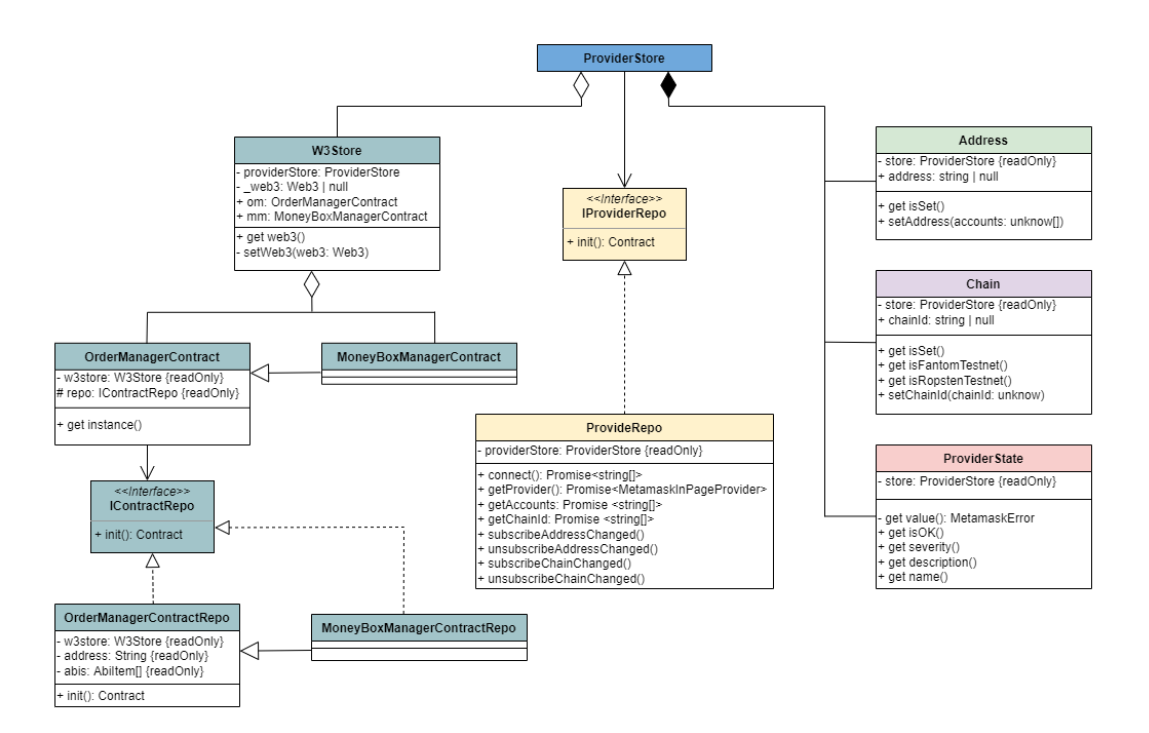
\includegraphics[scale = 0.5]{immagini/providerstore.png}
    \caption{La gerarchia di ProviderStore}
\end{figure}



\begin{figure}[H]
    \centering
    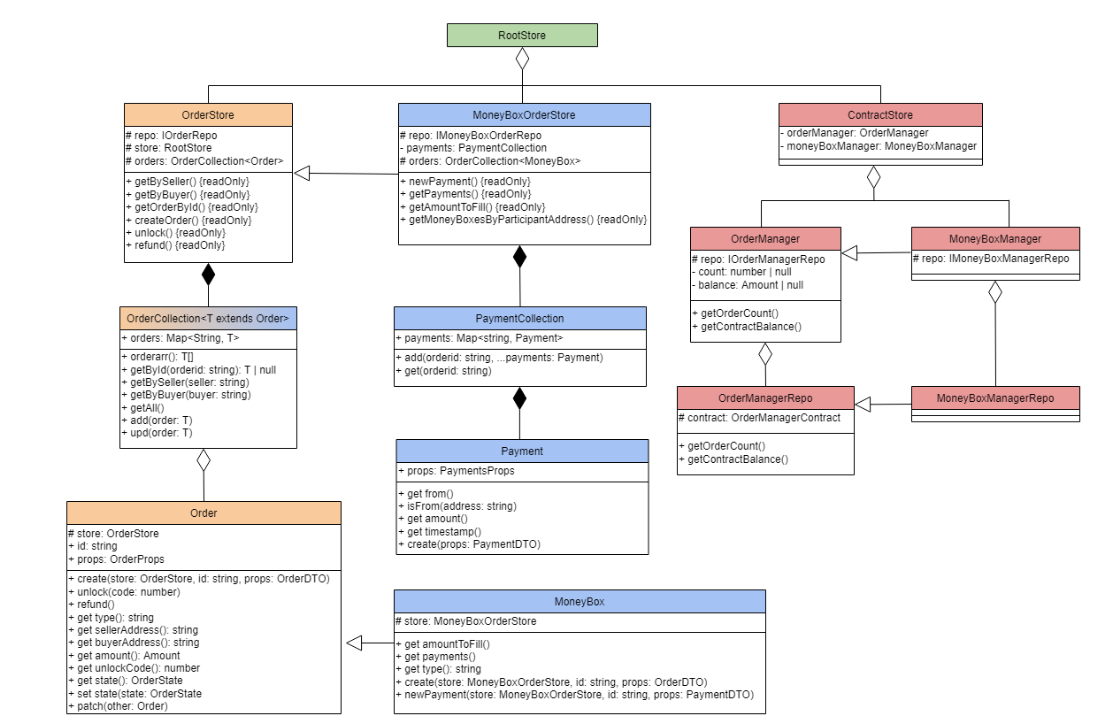
\includegraphics[scale = 0.5]{immagini/rootstore.png}
    \caption{Rootstore, le classi per gli ordini e la gestione dei contratti}
\end{figure}

\begin{landscape}
\begin{figure}[H]
    \centering
    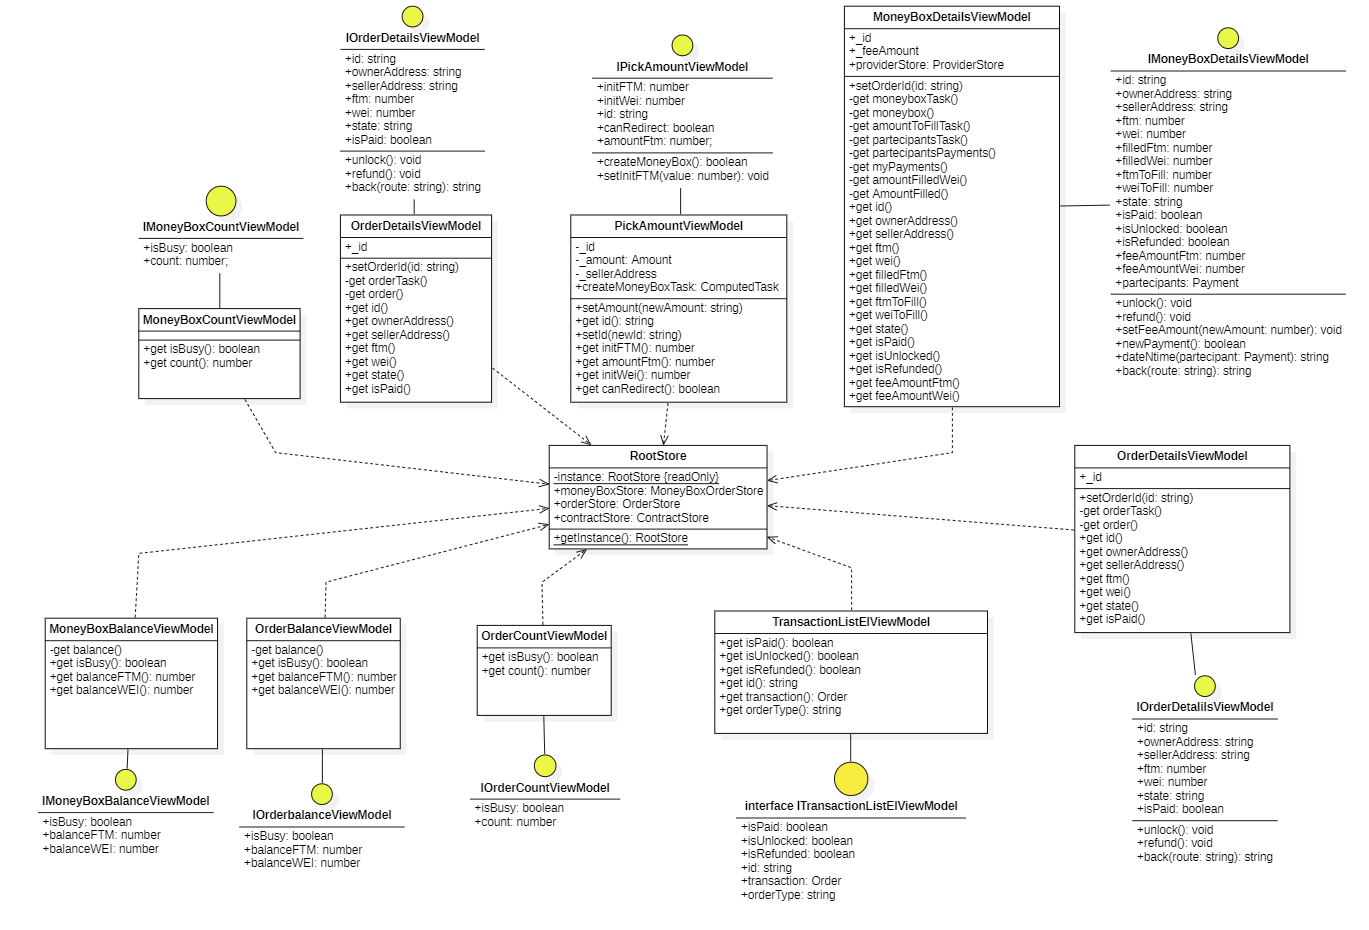
\includegraphics[scale = 0.6]{immagini/rsviewmodel.png}
    \caption{Le classi viewmodel dipendenti da RootStore}
\end{figure}
\end{landscape}

\subsubsection{Classi Solidity}

\begin{figure}[H]
    \centering
    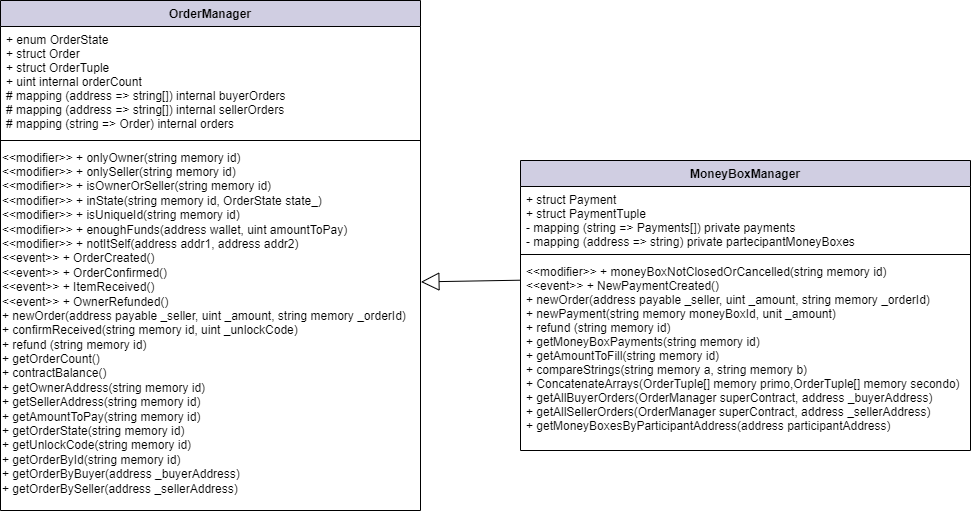
\includegraphics[scale = 0.45]{immagini/smartcontract.png}
    \caption{Le classi Solidity}
\end{figure}

Il diagramma delle classi Solidity, che gestiscono gli smartcontracts, è stato creato seguendo le indicazioni di \href{https://github.com/naddison36/sol2uml}{\textbf{sol2uml}}.
Esso è costituito da due classi:
\begin{itemize}
    \item \textbf{OrderManager}, si occupa della gestione di tutti i pagamenti singoli, salvati in più \textbf{map};
    \item \textbf{MoneyBoxManager}, si occupa della gestione delle Moneybox, anche esse mappate; essendo un'estensione di OrderManager, ne eredita tutti i metodi.
\end{itemize}
Tra i metodi, \textit{refund(string memory id)} si occupa di ritornare ai vari proprietari degli ordini 
(e a tutti i partecipanti nel caso di una MoneyBox) le somme di FTM interne al particolare contratto, identificato tramite \textit{id}.
\\
Per maggiori informazioni sulla parte dell'applicazione relativa alla Blockchain, si invita a consultare la sezione §\ref{section:blockchain}.



\subsection{Diagrammi di sequenza}

\begin{figure}[H]
    \centering
    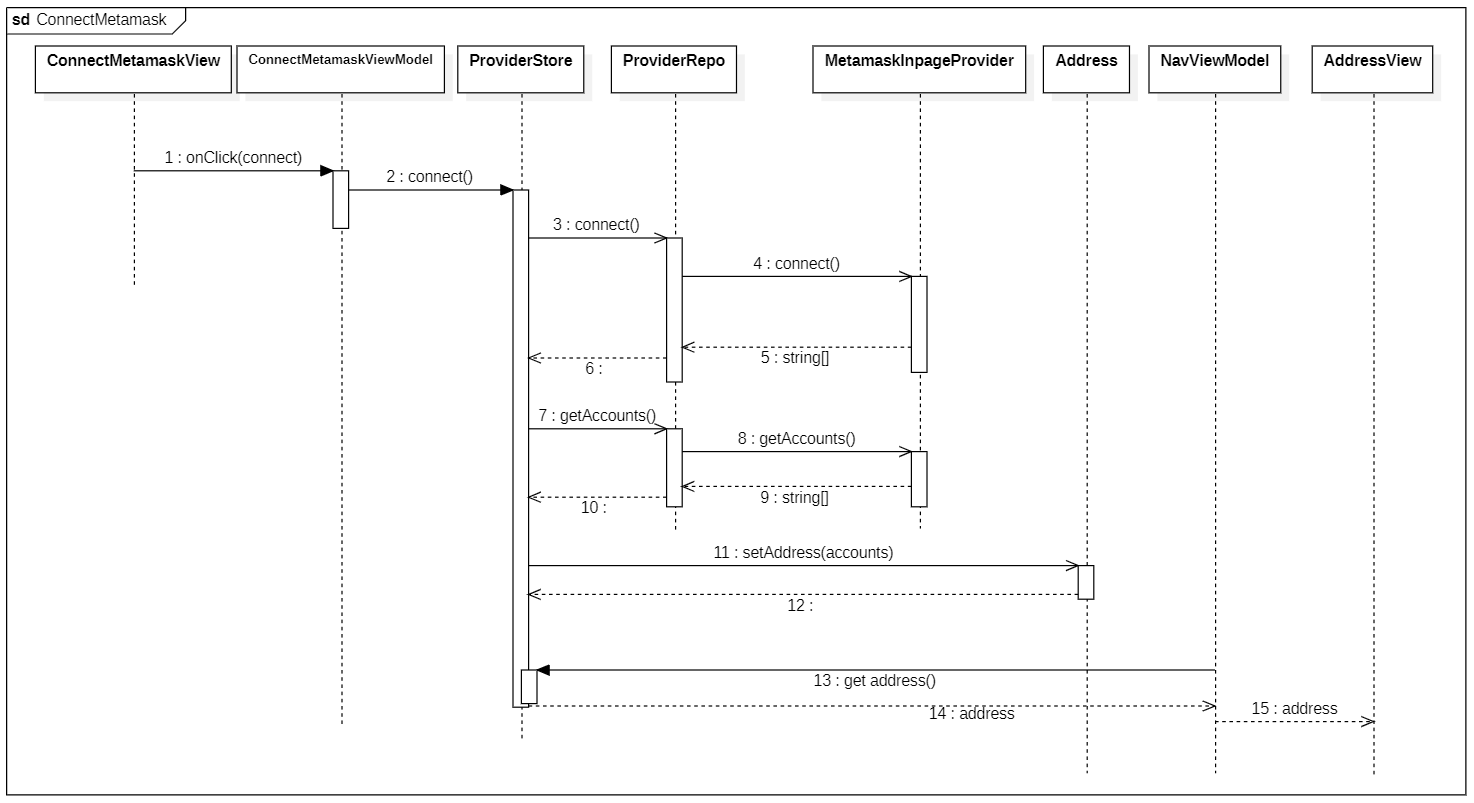
\includegraphics[scale = 0.45]{immagini/diagrammaMeta.png}
    \caption{Diagramma di sequenza per la connessione a Metamask}
\end{figure}

Il diagramma di sequenza sopra riportato è cosi descritto:

\begin{enumerate}
    \item La connessione a MetaMask inizia quando nella \textbf{ConnnectMetamaskView} mediante l'apposito pulsante viene fatto l'onclick e viene chiamato il metodo \textit{connect()} sul \textbf{ConnectMetamaskViewModel};
    \item Esso a sua volta chiama il metodo \textit{connect()} sul \textbf{ProviderStore} che a sua volta fa la chiamata asincrona del metodo \textit{connect} sul \textbf{ProviderRepo} che a sua volta fa la chiamata asincrona del metodo \textit{connect} su \textbf{MetamaskInpageProvider} e la connessione è così stabilita;
    \item Successivamente dato che potrebbero esserci più account connessi il \textbf{ProviderStore} chiama il metodo asincrono \textit{getAccounts} sul \textbf{ProviderRepo} che lo chiama a sua volta sul \textbf{MetaMaskInpageProvider}, il quale ritorna tutti gli indirizzi degli account connessi mediante un array di stringhe;
    \item Succcessivamente il \textbf{ProviderStore} setta l'indirizzo mediante il metodo \textit{setAddress} al quale viene passato in input il primo carattere dell'array di stringhe ritornato nel punto precedente;
    \item Infine la \textbf{NavViewModel} prende gli indirizzi connessi mediante il metodo \textit{getAddress} chiamato sul \textbf{ProviderStore}, e li ritorna alla \textbf{AddressView} per essere visualizzati.
\end{enumerate}

\begin{figure}[H]
    \centering
    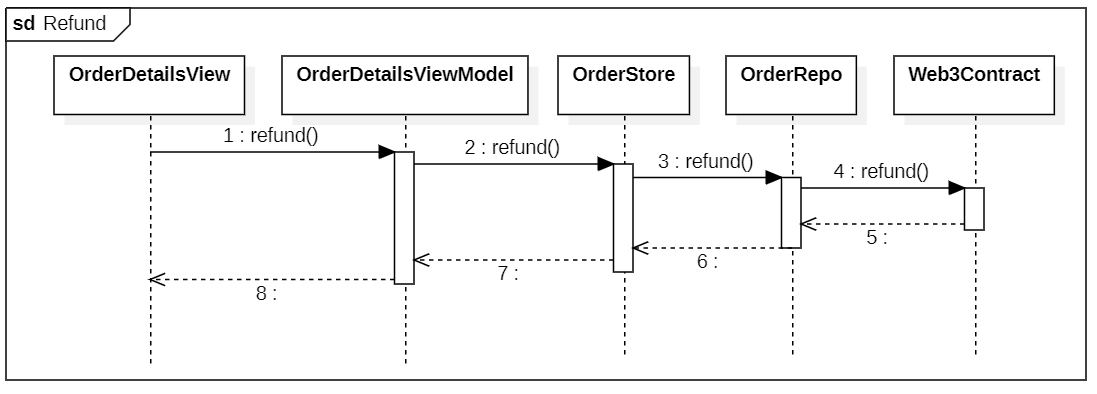
\includegraphics[scale = 0.6]{immagini/refund.png}
    \caption{Diagramma di sequenza della funzione di rimborso}
\end{figure}

Il diagramma di sequenza sopra riportato, molto semplice grazie ai pattern architetturali utilizzati, è cosi descritto:

\begin{enumerate}
    \item Dalla \textbf{OrderDetailsView}, dopo aver cliccato l'apposito bottone, parte la chiamata della funzione \textit{refund()} verso \textbf{OrderDetailsViewModel} per effettuare il rimborso dell'ordine corrente;
    \item Dal view-model, vengono chiamate le funzioni \textit{refund()} fino ad arrivare a Web3Contract, che si occuperà di contattare lo smartcontract nella Blockchain;
    \item Al ritorno delle varie funzioni, l'utente visualizzerà un messaggio di avvenuto rimborso dei pagamenti.
\end{enumerate}

\clearpage
\subsection{Architettura di dettaglio}

\subsubsection{Repository pattern}

Il repository pattern ci ha permesso di racchiudere tutte le interazioni con sorgenti esterne in un oggetto unico, mantenendo la separazione tra implementazione e interfaccia.

\subsubsection{Singleton}

Sono state implementate alcune classi seguendo il design pattern Singleton,
 ciò consente di garantire che una classe abbia una sola istanza, fornendo al contempo un punto di accesso globale alla stessa.
Il design singleton è stato usato per avere un'unica fonte detentrice dello stato di ogni modello.
Le classi più importanti create seguendo il pattern singleton sono:

\begin{itemize}
    \item \textbf{RootStore}: 
    \item \textbf{ProviderStore}: 
    \item \textbf{W3Store}: classe che gestisce la connessione a Metamask.
\end{itemize}

\subsubsection{Observer pattern}

Attraverso Mobx abbiamo usato l'observer pattern in quasi tutte le classi del frontend in modo tale che, alla modifica di una classe observable, i cambiamenti si rifletteranno nelle classi observer.
\section{Blockchain}\label{section:blockchain}

La nostra applicazione non fa uso di alcun backend in quanto sfrutta appieno le funzionalità della blockchain: 
sulla testnet Fantom sono stati infatti deployati i due smart contract utilizzati per i diversi tipo di pagamento.
Tutti i file dedicati alla blockchain si trovano nel repository \textbf{smart-contract}, consultabili e clonabili al seguente link:

\begin{center}
    \href{https://github.com/Yakuzaishi-SWE/smart-contract}{https://github.com/Yakuzaishi-SWE/smart-contract}
\end{center}

I file sono cosi organizzati:
\begin{itemize}
    \item \textit{test} è la sottocartella contenente i file \textbf{1\_OrderManager.test.js} e \textbf{2\_MoneyBox.test.js}, utili a controllare che tutte le funzionalità dei contratti siano corrette;
    \item \textit{contracts} è la sottocartella contenente i due smartcontract \textbf{OrderManager.sol} e \textbf{MoneyBoxManager.sol};
    \item il resto per midena?
\end{itemize}
\section{Conversione a Stable Coin}\label{section:conversione_stable}

La funzionalità di convertire l'ammontare depositato sul contratto in stable coin è un'interessante funzionalità che il gruppo ha individuato ed aggiunto ai requisiti.\\
Il gruppo ha condotto quindi uno studio relativamente ai passaggi da affrontare per attuare il meccanismo di conversione dei token\glo{}.
Prima di procedere è necessario descrivere e comprendere alcune componenti fondamentali che sono necessarie:

\begin{itemize}
    \item Wrapped FTM: è un token crypto ancorato al valore del Fantom. Viene chiamato così oerchè l'asset originale viene messo in un wrapper che consente di crearne una versione su un'altra blockchain. Questo permette di creare ponti tra diverse blockchain e utilizzare asset non nativi su  un'altra blockchain. Ovviamente in genere può essere riscattato per il corrispettivo in qualsiasi momento. Il processo di "wrapping" permette quindi di rendere il token Fantom conforme allo standard ERC-20 e poter essere, ad esempio nel nostro caso, convertito;
    \item Stable Coin: è un token che ha valore fissato con un rapporto 1:1 con una valuta FIAT\glo{};
    \item Liquidity Pool: è un insieme di fondi bloccati in uno smart contract che generalmente contengono due token diversi. Hanno diversi casi d'uso tra cui la possibilità di fungere da punto di scambio tra i due token;
    \item Factory Contract: è un contratto che si occupa di gestire ed eseguire oprazioni sulle coppie di token. In particolare la sua funzione principale è quella di creare uno smart contract associato alla coppia di token scelta. Quest'ultima funzione è necessaria se si vuole generare una propria liquidity pool;
    \item Router Contract: è un contratto che fornisce un supporto a tutte quelle che sono le funzionalità di trading dei token e gestione della liquidità.
\end{itemize}

Le componenti citate sono fondamentali per poter effettuare la conversione in stable coin. 
Il gruppo ha deciso di sviluppare un primo PoC di questa funzionalità direttamente sulla rete fantom di test. La rete di test presenta però delle mancanze rispetto alla rete principale, vengono a mancare infatti i contratti di alcuni token, come ad esempio USDT (scelto dal gruppo), e quelli che si occupa di gestire le liquidity pool di WFTM e eventuali stable coin.
Il gruppo ha deciso di creare un token che simuli il comportamento di USDT (è possibile visualizzare il contratto associato al seguente link):

\href{}{link}

Purtroppo non è possibile replicare il funzionamento di un vero USDT e il suo relativo vincolo al valore del dollaro, ma è sufficiente per dimostrare come avvenga il processo di conversione.\\

Sulla rete Fantom il provider dei contratti per la gestione delle coppie di token e delle pool di liquidità è SpookySwap. In particolare come anticipato, è necessario riferirsi ai due contratti UniswapV2Factory (Contract Factory) e UniswapV2Router02 (Contract Router), è possibile visualizzarne i riferimenti al seguente link della documentazione:

\begin{center}
    \href{https://docs.spooky.fi/Resources/contracts}{https://docs.spooky.fi/Resources/contracts}
\end{center}

Tramite il contratto UniswapV2Factory abbiamo creato la pair WFTM/USDT (usando il token ERC-20 da noi creato).\\ Dopo aver creato la coppia è stata generata la corrispondente liquidity pool in cui è possibile fornire o rimuovere liquidità. 
è importante ricordare che il valore del token USDT da noi creato è associato al rapporto delle quantità dei due token presenti nella pool e non al dollaro.\\

A questo punto abbiamo proceduto ad inserire all'interno del contratto la chiamata al contratto UniswapV2Router02 per effettuare la conversione tra i due token.
Il metodo da chiamare è UniswapV2Router02.swapETHForExactTokens, che prende in input:

\begin{itemize}
    \item Equivalente di USDT da richiedere alla pool;
    \item Array contente gli indirizzi dei due contratti dei due token;
    \item Indirizzo a cui ritornare gli USDT richiesti (in questo caso è necessario indicare l'indirizzo del contratto);
    \item Un timestamp che indichi il timeout dopo il quale la transazione deve essere annullata.
\end{itemize}

Per approfondire ulteriormente il metodo, si veda la relativa documentazione:

\begin{center}
    \href{https://docs.uniswap.org/protocol/V2/reference/smart-contracts/router-02\#swaptokensforexacttokens}{https://docs.uniswap.org/protocol/V2/reference/smart-contracts/router-02\#swaptokensforexacttokens}
\end{center}

Poiché la conversione viene effettuata dal router su una pool, che verrà utilizzata da più utenti, il valore della conversione può cambiare rapidamente anche solo di poco. Il router in tal caso tornerà un ammontare di FTM da restituire al mittente della transazione nel caso in cui la conversione sia a suo sfavore. è necessario tenere traccia di questo comportamento e gestire la restituzione di tale importo.

%{screen con il codice}


\section{Punti di estensione} \label{section:punti_estensione}

ShopChain è un'applicazione progettata pensando anche ad eventuali operazioni future di manutenzione o
estensione del prodotto: durante lo sviluppo dell'applicazione ShopChain sono stati esplorati vari spunti per nuove features e ampliamenti, 
che però a causa del poco tempo rimasto non sono state implementate in tempo.
Sono state individuate principalmente tre macro aree che potranno essere ampliate.

\subsection{Smart Contract}

\subsubsection{Conversione a stable coin}

La funzionalità di convertire l'ammontare depositato sul contratto in stable coin è un'interessante funzionalità che il gruppo ha individuato. Per limiti 
di tempo e costi legati al progetto, non è stata implementata in tutti i suoi punti, ma è stata affrontata sul lato smart contract.\\
Il gruppo ha condotto quindi uno studio relativamente ai passaggi da affrontare per attuare il meccanismo di conversione dei token\glo{}.
Prima di procedere è necessario descrivere e comprendere alcune componenti fondamentali che saranno necessarie:

\begin{itemize}
    \item Wrapped FTM: è un token crypto ancorato al valore del Fantom. Viene chiamato così oerchè l'asset originale viene messo in un wrapper che consente di crearne una versione su un'altra blockchain. Questo permette di creare ponti tra diverse blockchain e utilizzare asset non nativi su  un'altra blockchain. Ovviamente in genere può essere riscattato per il corrispettivo in qualsiasi momento. Il processo di "wrapping" permette quindi di rendere il token Fantom conforme allo standard ERC-20 e poter essere, ad esempio nel nostro caso, convertito;
    \item Stable Coin: è un token che ha valore fissato con un rapporto 1:1 con una valuta FIAT\glo{};
    \item Liquidity Pool: è un insieme di fondi bloccati in uno smart contract che generalmente contengono due token diversi. Hanno diversi casi d'uso tra cui la possibilità di fungere da punto di scambio tra i due token;
    \item Factory Contract: è un contratto che si occupa di gestire ed eseguire oprazioni sulle coppie di token. In particolare la sua funzione principale è quella di creare uno smart contract associato alla coppia di token scelta. Quest'ultima funzione è necessaria se si vuole generare una propria liquidity pool;
    \item Router Contract: è un contratto che fornisce un supporto a tutte quelle che sono le funzionalità di trading dei token e gestione della liquidità.
\end{itemize}

Le componenti citate sono fondamentali per poter effettuare la conversione in stable coin. 
Il gruppo ha deciso di sviluppare un primo PoC di questa funzionalità direttamente sulla rete fantom di test. La rete di test presenta però delle mancanze rispetto alla rete principale, vengono a mancare infatti i contratti di alcuni token, come ad esempio USDT (scelto dal gruppo), e quelli che si occupa di gestire le liquidity pool di WFTM e eventuali stable coin.
Il gruppo ha deciso di creare un token che simuli il comportamento di USDT (è possibile visualizzare il contratto associato al seguente link):

\href{}{link}

Purtroppo non è possibile replicare il funzionamento di un vero USDT e il suo relativo vincolo al valore del dollaro, ma è sufficiente per dimostrare come avvenga il processo di conversione.\\

Sulla rete Fantom il provider dei contratti per la gestione delle coppie di token e delle pool di liquidità è SpookySwap. In particolare come anticipato, è necessario riferirsi ai due contratti UniswapV2Factory (Contract Factory) e UniswapV2Router02 (Contract Router), è possibile visualizzarne i riferimenti al seguente link della documentazione:

\begin{center}
    \href{https://docs.spooky.fi/Resources/contracts}{https://docs.spooky.fi/Resources/contracts}
\end{center}

Tramite il contratto UniswapV2Factory abbiamo creato la pair WFTM/USDT (usando il token ERC-20 da noi creato).\\ Dopo aver creato la coppia è stata generata la corrispondente liquidity pool in cui è possibile fornire o rimuovere liquidità. 
è importante ricordare che il valore del token USDT da noi creato è associato al rapporto delle quantità dei due token presenti nella pool e non al dollaro.\\

A questo punto abbiamo proceduto ad inserire all'interno del contratto la chiamata al contratto UniswapV2Router02 per effettuare la conversione tra i due token.
Il metodo da chiamare è UniswapV2Router02.swapETHForExactTokens, che prende in input:

\begin{itemize}
    \item Equivalente di USDT da richiedere alla pool;
    \item Array contente gli indirizzi dei due contratti dei due token;
    \item Indirizzo a cui ritornare gli USDT richiesti (in questo caso è necessario indicare l'indirizzo del contratto);
    \item Un timestamp che indichi il timeout dopo il quale la transazione deve essere annullata.
\end{itemize}

Per approfondire ulteriormente il metodo, si veda la relativa documentazione:

\begin{center}
    \href{https://docs.uniswap.org/protocol/V2/reference/smart-contracts/router-02\#swaptokensforexacttokens}{https://docs.uniswap.org/protocol/V2/reference/smart-contracts/router-02\#swaptokensforexacttokens}
\end{center}

Poichè la conversione viene effettuata dal router su una pool, che verrà utilizzata da più utenti, il valore della conversione può cambiare rapidamente anche solo di poco. Il router in tal caso tornerà un ammontare di FTM da restituire al mittente della transazione nel caso in cui la conversione sia a suo sfavore. è necessario tenere traccia di questo comportamento e gestire la restituzione di tale importo.

%{screen con il codice}


\subsubsection{TheGraph protocol}

Nella pagina di visualizzazione degli ordini il gruppo ha implementato la possibilità di filtrare gli ordini restituiti direttamente dalla blockchain. Attualmente questa funzionalità è fornita solo tramite un controllo a front-end, in futuro si potrebbe evolvere la funzione di filtraggio tramite l'implementazione del protocollo TheGraph\glo.

The Graph è un protocollo decentralizzato per indicizzare e successivamente effettuare query dei dati presenti in blockchain in una modalità simile a quella che avviene con una normale base di dati. Questo permette di interrogare la blockchain in modo facile e veloce, ed estraendo dati che altrimenti non sarebbe possibile visualizzare.

In particolare quanto citato è possibile tramite la creazione di subgraph. Un sottografo non è altro che una serie di parametri necessari al protocollo per poter mappare e creare un indice dei dati presenti in blockchain.\\
Si compongono di tre componenti principali:

\begin{itemize}
 \item Manifest (subgraph.yaml) che definisce quali dati il sottografo andrà a indicizzare;

 \begin{figure}[H]
    \centering
    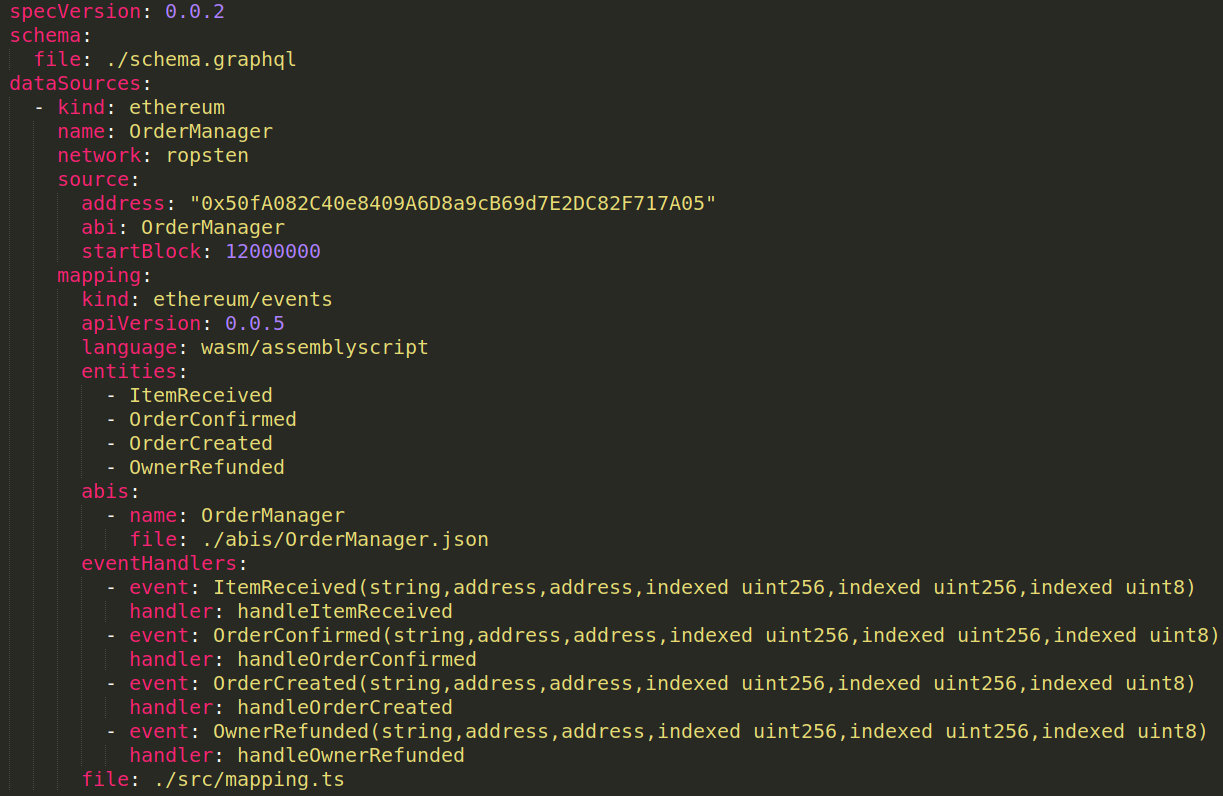
\includegraphics[scale=0.3]{immagini/subgraf.png}
    \caption{Esempio di un possibile subgraph configurato per il contratto OrderManager per la rete Ropsten.}
 \end{figure}


 \item Schema (schema.graphql) che riporta quali dati si desiderà ricevere dal sottografo;

 \begin{figure}[H]
    \centering
    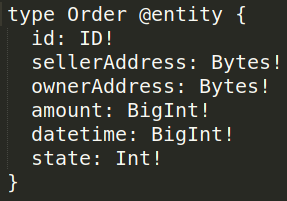
\includegraphics[scale=0.4]{immagini/schema.png}
    \caption{Esempio di file schema per la definizione entità Order.}
 \end{figure}

 \item AssemblyScript Mappings (mapping.ts) file che riporta la traduzione dei dati presenti in blockchain che il sottografo dovrà indicizzare.

 \begin{figure}[H]
    \centering
    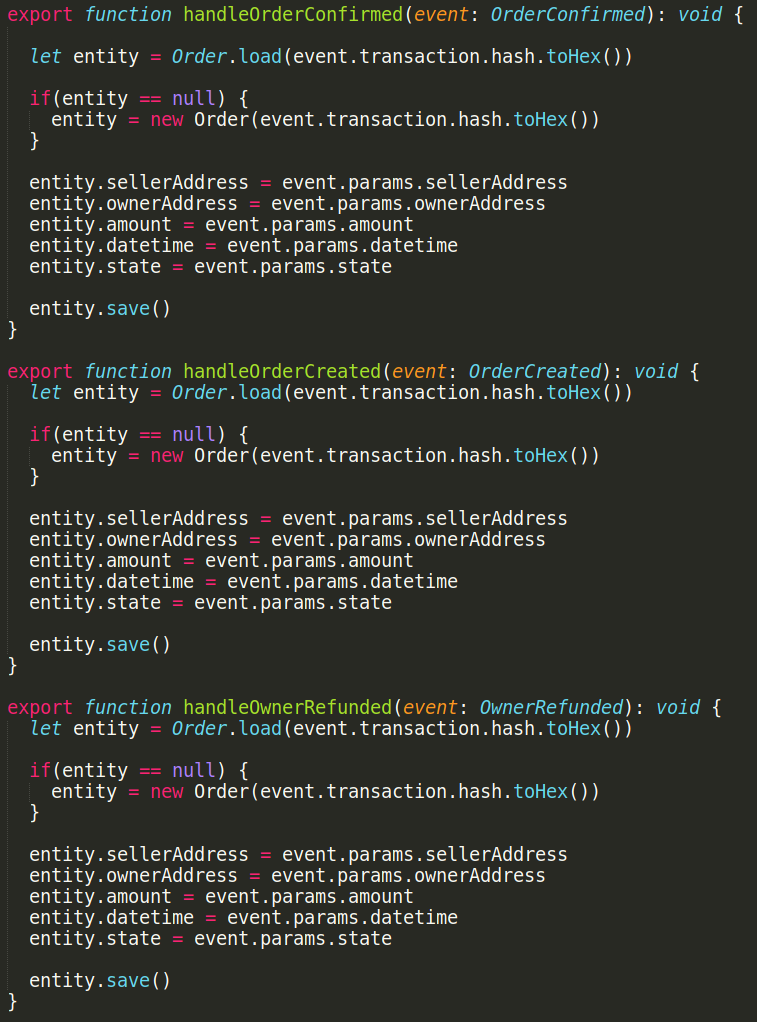
\includegraphics[scale=0.3]{immagini/map.png}
    \caption{Esempio di file mapping per l'indicizzazione degli eventi.}
 \end{figure}

\end{itemize}

Questa funzionalità non è stata portata avanti perchè non è disponibile sulla testnet di Fantom, ma solo sulla mainnet. Se la si vuole implementare sarà quindi necessario eseguire lo sviluppo e i relativi test su una testnet di Ethereum in cui è disponibile il protocollo (es. Rinkeby\glo). Una volta che lo sviluppo sarà finito si potrà procedere a caricare il subgraph creato sulla mainnet di Fantom senza particolari modifiche, poichè quest'ultima è una blockchain EVM.


\subsection{Chain differenti}

Un ovvio ampliamento per l'applicazione è il supporto a più blockchain, per raggiungere un bacino di utenza più ampio e garantire quindi un maggior successo dell'applicazione.\\


\subsection{Frontend}

\subsubsection{Immagine MoneyBox}

Il gruppo aveva pensato di associare ad ogni MoneyBox una immagine generata automaticamente, o presa da un pool di immagini definito. Se si sceglie di generarla automaticamente, si può prendere come seed di generazione uno tra i seguenti: l'id dell'ordine associato alla MoneyBox, 
il numero del blocco relativo alla transazione in blockchain, il timestamp della creazione.
Questo contribuisce ad una maggiore sicurezza nel condividere il link alla suddetta MoneyBox con amici, che potranno vedere a colpo d'occhio se il link è corretto tramite l'immagine incorporata.

\subsubsection{Riflettere i cambiamenti del contratto}

Con i cambiamenti che possono venire apportati agli smartcontract è bene che il lato frontend dell'applicazione sia aggiornato di conseguenza.
Nel caso dei cambiamenti proposti finora i cambiamenti individuati sono i seguenti:
\begin{itemize}
    \item \textbf{Stable Coin}: nelle pagine di pagamento, di dettaglio dell'ordine e di dettagli della MoneyBox, viene mostrato anche l'ammontare in stable coin dei vari pagamenti, per una migliore visione dei costi da parte dell'utente;
    \item \textbf{TheGraph}: le due pagine di elenco transazioni dovranno essere modificate per sfruttare appieno tutte le funzionalità portate dalla implementazione dei protocolli TheGraph;
    \item \textbf{Chain differenti}:  in un pop-up all'ingresso dell'applicazione, l'utente potrà selezionare la chain (e quindi la cryptovaluta correlata) con la quale procedere al pagamento. Tale scelta dovrà essere riportata anche nella breadcrumb come reminder testuale.
\end{itemize}


\newglossaryentry{Criptovaluta}
{
  name={Criptovaluta},
  description={Traduzione in italiano del termine inglese cryptocurrency e si riferisce ad una rappresentazione digitale di valore basata sulla crittografia. Si tratta di una risorsa digitale paritaria e decentralizzata. Al mondo esistono oltre 13000 criptovalute.}
}

\newglossaryentry{E-Commerce}
{
  name={E-Commerce},
  description={Insieme di attività di vendita e acquisto di prodotti effettuato tramite internet.}
}

\newglossaryentry{Smart contract}
{
  name={Smart contract},
  description={Sono essenzialmente dei programmi salvati sulla blockchain che convertono i tradizionali contratti nella loro controparte digitale. Hanno quindi il vero e proprio obiettivo di digitalizzare i termini di un accordo in codice che viene eseguito quando i termini del contratto vengono rispettati.}
}

\newglossaryentry{Wallet}
{
  name={Wallet},
  description={Letteralmente un portafoglio per le criptovalute, che si traduce fisicamente in un dispositivo, un supporto fisico, un programma o un servizio che memorizza le chiavi pubbliche e/o private per le transazioni di criptovaluta.}
}

\newglossaryentry{Fantom}
{
  name={Fantom},
  description={Blockchain relativamente recente nata nel dicembre 2019 e si basa su un proprio algoritmo di consenso personalizzato. Vanta come punto di forza la velocità relativa alle transazioni, dichiara inferiore ai due secondi dagli sviluppatori stessi.}
}

\newglossaryentry{FTM}
{
  name={FTM},
  description={Simbolo di valuta di Fantom.}
}

\newglossaryentry{Blockchain}
{
  name={Blockchain},
  description={Letteralmente significa "catena di blocchi", è una struttura dati decentralizzata i cui dati sono raggruppati in blocchi concatenati in ordine cronologico e la cui integrità è garantita dall'uso della crittografia. Il suo contenuto è "immutabile". Una volta scritto tramite un processo normato non è più modificabile né eliminabile, a meno di non invalidare l'intero processo.}
}

\newglossaryentry{Observer}
{
  name={Observer},
  description={È l’oggetto osservatore nel design pattern Observer\glo.}
}

\newglossaryentry{Observable}
{
  name={Observable},
  description={È l’oggetto osservato nel design pattern Observer\glo, detto anche ”Subject”.}
}

\newglossaryentry{Observer design pattern}
{
  name={Observer design pattern},
  description={È un design pattern software utilizzato per far si che un oggetto observable\glo\ (”osservato”) notifichi modifiche interne all’observer\glo\ (”osservatore”), che reagirà di conseguenza, solitamente chiamando un suo metodo interno.}
}

\newglossaryentry{Repository}
{
  name={Repository},
  description={Ambiente di un sistema informativo, in cui vengono gestiti i metadati, attraverso tabelle relazionali; l’insieme di tabelle, regole e motori di calcolo tramite cui si gestiscono i metadati prende il nome di metabase.}
}

\newglossaryentry{Git}
{
  name={Git},
  description={Software di controllo di versione distribuito utilizzabile da interfaccia a riga di comando, creato da Linus Torvalds nel 2005.}
}

\newglossaryentry{GitHub}
{
  name={GitHub},
  description={Servizio di hosting per sviluppatori. Fornisce uno strumento di controllo versione e permette lo sviluppo distribuito del software.}
}

\newglossaryentry{Pattern architetturale}
{
  name={Pattern architetturale},
  description={È una modellazione architetturale di un prodotto software. Ne esistono diversi e permettono di separare il comportamento delle componenti che lo compongono, aumentando il disaccoppiamento e favorendo lo unit-test delle varie componenti.}
}

\newglossaryentry{Model-View-Controller(MVC)}
{
  name={Model-View-Controller(MVC)},
  description={Pattern architetturale molto diffuso nello sviluppo di software. Consiste nel dividere il prodotto in tre parti fondamentali: il modello, il controller, e la vista. Il controller si occupa di far comunicare vista e modello, ricevendo gli input dell’utente attraverso la vista e avvisando il modello dei cambiamenti avvenuti. La view in questo caso è in grado di visualizzare direttamente i dati contenuti nel modello.}
}

\newglossaryentry{Model-View-ViewModel(MVVM)}
{
  name={Model-View-ViewModel(MVVM)},
  description={Pattern architetturale derivato dal Model-View-Controller(MVC)\glo\ che prevede l’utilizzo di un View-Model per far comunicare vista e modello. In questo caso la vista non ha alcuna comunicazione con il modello quindi il disaccoppiamento è maggiore rispetto a MVC.}
}

\newglossaryentry{Stato interno}
{
  name={Stato interno},
  description={Un componente React può possedere uno stato interno (statefull) oppure no (stateless). Questo stato è un insieme più o meno numeroso di dati, i quali possono essere modificati attraverso interazioni dell’utente con questo componente (nella vista). La modifica di tali dati causa la rirenderizzazione del componente stesso e dei suoi figli.}
}

\newglossaryentry{Metamask}
{
  name={Metamask},
  description={Metamask è un software wallet per criptovalute usato per interagire con la blockchain Ethereum. Esso lascia accedere gli utenti ai loro walllet Etherium tramite un'estensione browser o una app mobile, che sono poi usate per interagire con applicazioni decentralizzate.}
}

\newglossaryentry{Docker}
{
  name={Docker},
  description={È una piattaforma open source di "containerizazzione": permette agli sviluppatori di racchiudere applicazioni in "container", componenti eseguibili standardizzati che uniscono il codice sorgente dell'app con le librerie di sistema e le dipendenze richieste per eseguire quel codice in qualsiasi ambiente.}
}

\newglossaryentry{BIOS}
{
  name={BIOS},
  description={È il firmware utilizzato per fornire servizi runtime ai sistemi operativi e programmi, e per eseguire l'Inizializzazione hardware durante lo start-up della macchina.}
}

\newglossaryentry{DApp}
{
  name={DApp},
  description={È un'applicazione che può operare autonomamente, tipicamente tramite l'uso di smartcontracts eseguiti su una blockchain completamente decentralizzata.}
}

\newglossaryentry{MobX}
{
  name={MobX},
  description={È una libreria per gestire in modo reattivo gli stati di una applicazione. Nonostante sia usabile in modo indipendente da React, sono comunemente usati assieme.}
}

\newglossaryentry{Testnet}
{
  name={Testnet},
  description={Nel gergo crypto, una testnet è una istanza di una blockchain usata per testing e sperimentazioni, senza il rischio di pagamenti e di intaccare la rete principale. Le cryptovalute delle testnet sono diverse da quelle delle reti principali, non hanno valore, e sono gratuitamente ottenibili.}
}

\newglossaryentry{Stable Coin}
{
  name={Stable Coin},
  description={Una criptovaluta con un valore che riflette completamente quello di una valuta reale, molto spesso il dollaro, per garantire una maggiore stabilità nelle transazioni.}
}

\newglossaryentry{TheGraph}
{
  name={TheGraph},
  description={È un protocollo di indicizzazione per organizzare dati blockchain e renderli facilmente accessibili tramite GraphQL\glo.}
}

\newglossaryentry{GraphQL}
{
  name={GraphQL},
  description={Linguaggio open source per richieste e manipolazione di dati per APIs\glo, è stata rilasciata pubblicamente nel 2015.}
}

\newglossaryentry{API}
{
  name={API},
  description={Le API, Application Programming Interface, sono connessioni tra diversi computers o tra diversi programmi, e definiscono come le parti comunicano tra loro tramite richieste e risposte.}
}

\newglossaryentry{Rinkeby}
{
  name={Rinkeby},
  description={Una delle due maggiori testnet\glo\ Etherium.}
}

\newglossaryentry{Token}
{
  name={Token},
  description={Un token è }
}

\newglossaryentry{FIAT}
{
  name={FIAT},
  description={Le FIAT sono valute emesse da un governo che sono supportate da un corrispettivo ammontare di un bene tangibile, molto spesso l'oro).}
}

\newglossaryentry{DAL}
{
  name={DAL},
  description={Un Data Access Layer (DAL) è un layer di un programma che fornisce un accesso semplificato ai dati memorizzati in una memoria persistente di qualche tipo, come ad esempio un database entità-relazionale.}
}

\newglossaryentry{Dependency Injection}
{
  name={Dependency Injection},
  description={In ingegneria software, la dependency injection è un design pattern in cui un oggetto contiene altri oggetti da cui dipende.}
}
	%%%%%%%%%%%%%%%%%%%%%%%%%%%%%%%%%%%%%%%%%%%%%%%%%%%%%%%%%%%%%%%
\end{document}
